\chapter{Gravitational waves}\label{ch:gw}

The first observation of gravitational waves in 2015~\citep{gw150914} took place a century after Albert Einstein completed his general theory of relativity~\citep{Einstein_1916}.
Einstein's original publication proposed that gravitational attraction was not mediated by a force as described by Newtonian physics, but rather it was caused by the curvature of space-time due to the presence of mass.
He primarily discussed the relevance of general relativity to predicting gravitational redshift, the curvature of light rays, and the perihelion precession of the orbit of Mercury, a mystery that perplexed late nineteenth and early twentieth century astronomers.
However, the idea that gravitational forces might propagate in the form of waves similar to electromagnetic waves had existed since it was first speculated by Henri Poincar\'e a decade prior~\citep{Poincare_1905}, and Einstein would soon make the conjecture that his theory of general relativity could provide a robust mathematical framework for gravitational waves.

Initially, Einstein was not highly confident in his conjecture.
Electromagnetic waves are typically produced in the form of dipole radiation, formed by a positive and negative electric charge, whereas no ``negative mass'' exists to produce an analogous gravitational dipole.
His early efforts in making approximations to his field equations to yield wave-like solutions were mostly fruitless due to the complexity of the equations.
Nevertheless progress made by Einstein and his collaborators over the following decades would culminate in a theory for gravitational radiation propagating as transverse waves that squeeze and stretch matter perpendicular to the direction of propagation.

This chapter gives an overview of the theoretical background necessary for understanding the emission of \acp{GW} (Section~\ref{sec:gw-gr}), following discussions from \citet{Creighton_2011}, \citet{Hartle_2003}, \citet{Jaranowski_2009}, and \citet{Misner_1973}, and describes known and expected sources of \ac{GW} radiation (Section~\ref{sec:gw-sources}).


\section{General Relativity}\label{sec:gw-gr}

In Newtonian mechanics, gravitational attraction is described as the manifestation of a gravitational potential $\Phi$ generated by a source of mass density $\rho$:
\begin{equation}
	\nabla^2 \Phi = 4\pi\rho.
\end{equation}
General relativity relates the geometry of spacetime to the density and flux of energy and momentum through the Einstein field equations
\begin{equation}\label{eq:gr-einstein}
	G_{\mu\nu} = \frac{8\pi G}{c^4} T_{\mu\nu}
\end{equation}
where $G_{\mu\nu}$ is the Einstein tensor, analogous to the Newtonian potential $\Phi$, and $T_{\mu\nu}$ is the energy-momentum tensor, analogous to $\rho$.
Since the tensors are 4-by-4 and symmetric, \cref{eq:gr-einstein} represents ten separate equations, as opposed to the single Newtonian equation.
The energy-momentum tensor represents not just the mass density (which is described by the $T^{00}$ component alone) but also the momentum density ($T^{i0}$ and $T^{0j}$ terms, where $i,j = 1, 2, 3$) and the mechanical stress tensor ($T^{ij}$).

To unpack $G_{\mu\nu}$ we have to define some basic quantities of general relativity.
The geometry of spacetime is described by the metric tensor $g_{\mu\nu}$, via the relationship between the coordinate distances and the line element:
\begin{equation}
	ds^2 = g_{\mu\nu}dx^{\mu}dx^{\nu}.
\end{equation}
% In a flat Minkowski spacetime, where the metric is
% \begin{equation}
% 	\eta_{\mu\nu} = \left(
% 			\begin{matrix}
% 				-1 & 0 & 0 & 0\\
% 			  0 & 1 & 0 & 0\\
% 				0 & 0 & 1 & 0\\
% 				0 & 0 & 0 & 1\\
% 			\end{matrix}
% 		\right)
% \end{equation}
% the line element is that of special relativity: $ds^2 = -cdt^2 + dx^2 + dy^2 + dz^2$.s
Analogous to Newton's laws of motion in classical mechanics, the geodesic equations dictate how free-falling particles in general relativity move through spacetime along geodesics
\begin{equation}\label{eq:gr-geodesic}
	\frac{d^2x^{\mu}}{ds^2} + \Gamma_{\alpha \beta}^{\mu} \frac{dx^{\alpha}}{ds} \frac{dx^{\beta}}{ds} = 0
\end{equation}
where
\begin{equation}\label{eq:gr-christoffel}
	\Gamma_{\alpha \beta}^{\mu} = \frac{1}{2} g^{\mu\nu} \left( \partial_{\alpha} g_{\beta\nu} + \partial_{\beta} g_{\nu\alpha} - \partial_{\nu} g_{\alpha\beta} \right)
\end{equation}
are called the Christoffel symbols.
\Crefrange{eq:gr-geodesic}{eq:gr-christoffel} can be derived by asserting that vectors remain unchanged under parallel transport from one point to another within the spacetime described by $g_{\mu\nu}$.
The Christoffel symbols thus encode the effects of curvature on otherwise straight paths; note that in rectilinear coordinates they vanish and \cref{eq:gr-geodesic} reduces to the equation for a straight line.

A useful quantity is the Riemann curvature tensor
\begin{equation}\label{eq:gr-riemann}
	R_{\mu\nu\rho\sigma} = g_{\rho\lambda} \left(
		\partial_{\mu} \Gamma^{\lambda}_{\nu\sigma}
		- \partial_{\nu} \Gamma^{\lambda}_{\mu\sigma}
		+ \Gamma^{\lambda}_{\mu\eta} \Gamma^{\eta}_{\nu\sigma}
		- \Gamma^{\lambda}_{\nu\eta} \Gamma^{\eta}_{\mu\sigma}
	\right)
\end{equation}
from which we can define the Ricci tensor and its trace, the Ricci scalar:
\begin{equation}\label{eq:gr-ricci-tensor}
	R_{\mu\nu} = g^{\rho\sigma} R_{\rho\mu\sigma\nu}
\end{equation}
\begin{equation}\label{eq:gr-ricci-scalar}
	R = g^{\mu\nu} R_{\mu\nu}
\end{equation}
The Einstein tensor from \cref{eq:gr-einstein} can be written in terms of these quantities and the metric:
\begin{equation}\label{eq:gr-G}
	G_{\mu\nu} = R_{\mu\nu} - \frac{1}{2} R g_{\mu\nu}
\end{equation}

\subsection{Linear gravity}

We define our coordinate system such that the metric can be expressed as the flat Minkowski metric $\eta_{\mu\nu}$ plus a small perturbation $\abs{h_{\mu\nu}} \ll 1$: $g_{\mu \nu} = \eta_{\mu \nu} + h_{\mu \nu}$.
This allows us to develop a linearized form of the field equations, which we can then solve to arrive at a theory of \textit{weak} gravitational radiation.
The Christoffel symbols become
\begin{equation}\label{eq:gr-christoffel-lin}
	\Gamma_{\alpha \beta}^{\mu} = \frac{1}{2} \eta^{\mu\nu} \left( \partial_{\alpha} h_{\beta\nu} + \partial_{\beta} h_{\nu\alpha} - \partial_{\nu} h_{\alpha\beta} \right) + \order{h^2}.
\end{equation}
Combining these with \cref{eq:gr-riemann} gives the linearized Riemann tensor:
\begin{equation}\label{eq:gr-riemann-lin}
	R_{\mu\nu\rho\sigma} = \frac{1}{2} \left(
		\partial_{\rho} \partial_{\nu} h_{\mu \sigma}
		+ \partial_{\sigma} \partial_{\mu} h_{\nu \rho}
		- \partial_{\sigma} \partial_{\nu} h_{\mu \rho}
		- \partial_{\rho} \partial_{\mu} h_{\nu \sigma}
		+ \order{h^2}
	\right).
\end{equation}
Thus we can write the linearized Ricci tensor
\begin{equation}\label{eq:gr-ricci-tensor-lin}
	R_{\mu\nu} = \frac{1}{2} \left(
		\partial_{\alpha} \partial_{\mu} h_{\nu}^{\alpha}
		+ \partial_{\alpha} \partial_{\nu} h_{\mu}^{\alpha}
		- \partial_{\mu} \partial_{\nu} h
		- \Box h_{\mu\nu}
		+ \order{h^2}
	\right)
\end{equation}
and Ricci scalar
\begin{equation}\label{eq:gr-ricci-scalar-lin}
	R = \eta_{\mu\nu}R^{\mu\nu} = \partial_{\mu}\partial_{\nu}h - \Box h_{\mu\nu} + \order{h^2}
\end{equation}
where $h = \eta^{\mu\nu}h_{\mu\nu}$ is the trace of of the metric perturbation and $\Box$ is the Minkowski-spacetime D'Alembertian operator:
\begin{equation}
	\Box \vcentcolon= \eta^{\mu\nu} \partial_{\mu} \partial_{\nu} = -\frac{1}{c^2} \partial_t^2 + \partial_x^2 + \partial_y^2 + \partial_z^2.
\end{equation}
This yields the linearized Einstein tensor
\begin{equation}\label{eq:gr-einstein-lin}
	G_{\mu\nu} =
		\frac{1}{2} \left( \partial_{\mu}\partial_{\sigma}\Bar{h}_{\nu}^{\rho}
		+ \partial_{\nu}\partial_{\sigma}\Bar{h}_{\mu}^{\rho}
		- \Box \Bar{h}_{\sigma \rho}
		- \eta_{\mu\nu}\partial_{\sigma}\partial_{\rho}\Bar{h}^{\sigma\rho} \right)
		+ \order{h^2}
\end{equation}
where $\Bar{h}_{\mu\nu} := h_{\mu\nu} - \frac{1}{2}\eta_{\mu\nu}h$ is the trace-reversed metric perturbation (called so because its trace is $\Bar{h} = -h$).

We can simplify these terms further by choosing the appropriate gauge.
To do so we must first investigate how $g_{\mu\nu}$ behaves under a gauge transformation.
Suppose we make a small transformation to the coordinate system
\begin{equation}
	x^{\alpha} \rightarrow x'^{\alpha} = x^{\alpha} + \xi^{\alpha}.
\end{equation}
The metric transforms as
\begin{align}
	g_{\alpha\beta} \rightarrow g'_{\alpha\beta}
		&= \frac{\partial x^{\mu}}{\partial x'^{\alpha}} \frac{\partial x^{\nu}}{\partial x'^{\beta}} g_{\mu\nu}(x) \\
		&= g_{\alpha\beta} - \partial_{\alpha} \xi_{\beta} - \partial_{\beta} \xi_{\alpha} + \order{(\partial \xi)^2}.
\end{align}
or in terms of the metric perturbation,
\begin{equation}
	g'_{\alpha\beta} = \eta_{\alpha\beta} + h_{\alpha\beta} - \partial_{\alpha} \xi_{\beta} - \partial_{\beta} \xi_{\alpha} + \order{h (\partial \xi), (\partial \xi)^2}.
\end{equation}
We can write this as $g'_{\alpha\beta} = \eta_{\alpha\beta} + h'_{\alpha\beta} + \order{h (\partial \xi), (\partial \xi)^2}$,
from which we see how the perturbation has transformed:
\begin{equation}
	h'_{\alpha\beta} = h_{\alpha\beta} - \partial_{\alpha} \xi_{\beta} - \partial_{\beta} \xi_{\alpha}
\end{equation}
Trace-reversing again, we get
\begin{equation}
	\Bar{h}'_{\alpha\beta} = \Bar{h}_{\alpha\beta} - \partial_{\alpha} \xi_{\beta} - \partial_{\beta} \xi_{\alpha} + \eta_{\alpha\beta} \eta^{\mu\nu} \partial_{\mu} \xi_{\nu}.
\end{equation}

Analogous to the Lorenz gauge choice in electromagnetism, we assert the condition $\partial_{\alpha} \Bar{h}^{\alpha\beta} = 0$ in this gauge and find $\xi$ must satisfy
\begin{equation}
	\Box \xi_{\beta} = \partial_{\mu} \Bar{h}^{\mu}_{\beta}.
\end{equation}
Indeed solutions to this exist, therefore we are safe to make the gauge transformation.
The Lorenz gauge condition is chosen because it results in the divergence terms (all but the $\Box$ term) of \cref{eq:gr-einstein-lin} vanish.
In doing so, we reduce the linearized Einstein field equations to simply
\begin{equation}\label{eq:gr-linear}
	-\Box \Bar{h}_{\mu\nu} + \order{h^2} = \frac{16\pi G}{c^4} T_{\mu\nu}.
\end{equation}

In the Newtonian (slowly-varying) limit, the D'Alembertian operator becomes a spatial Laplace operator, and it can be shown~\citep{Creighton_2011} that the trace-reversed perturbation reduces to the Newtonian gravitational potential $\Phi$ and the energy-momentum tensor reduces to just the mass density, recovering the Poisson equation for Newtonian gravity: $\nabla^2\Phi = 4\pi G\rho$.


\subsection{Gravitational wave solutions}

In vacuum, the energy-momentum tensor is zero so the field equation is simply $\Box\Bar{h}_{\mu\nu}=0$, the solution to which is a monochromatic plane wave propagating at the speed of light:
\begin{equation}
	\Bar{h}_{\mu\nu} = A_{\mu\nu}\cos\left(k_\sigma x^\sigma - \phi_{\mu\nu}\right)
\end{equation}
where $A_{\mu\nu}$ and $\phi_{\mu\nu}$ are the amplitude and phase of the wave.
The 4-vector $k^{\mu}$ contains the frequency $k^0 = -\omega = -2\pi f$ and the wave vector $\mathbf{k}$ pointing in the direction of propagation.
The Lorenz gauge condition can now be expressed as $0 = \partial_{\mu} \Bar{h}^{\mu\nu} = -k_{\mu} A^{\mu\nu} \sin (k_{\alpha} x^{\alpha})$, which is satisfied if
\begin{equation}\label{eq:gr-transverse}
	k_{\mu} A^{\mu\nu} = 0.
\end{equation}
This means that the plane wave only has components orthogonal to $k_{\mu}$, i.e. it is transverse wave.
Furthermore, \cref{eq:gr-transverse} sets four conditions on what was originally ten components, so our choice of the Lorenz gauge has reduced the number independent components in the solution to six.

In the slowly-varying case the gauge condition can be further restricted by making the metric perturbation purely spatial, ($h_{00}=h_{0i}=0$) and traceless ($h=h_i^i$=0).
In this \textit{transverse-traceless (TT) gauge}, we write the metric perturbation as $h_{\mu\nu}^{TT}$ (no overline necessary because in this gauge $\Bar{h}_{\mu\nu} = h_{\mu\nu}$).
These gauge conditions again reduce the number of components by four, so now the solution has only two independent components.
For a monochromatic plane wave propagating in the $z$ direction, these two components are
\begin{align}
	h_{11}^{TT} &= -h_{22}^{TT} = h_+(t) \\
	h_{12}^{TT} &= h_{21}^{TT} = h_{\times}(t)
\end{align}
and are called the plus and cross polarizations, respectively.
The effect of these polarizations on an array of test particles is a stretching and compressing of the distances between the particles in the $xy$-plane.
This gives us a means of observing a gravitational wave:
measuring the distances between two ``test masses'' along one axis and between two separate test masses along another axis perpendicular to first.

To determine the energy emitted by gravitational waves, we must consider a source, i.e. a non-zero energy-momentum tensor.
This requires a general solution to \cref{eq:gr-linear}.
To do so we define an \textit{effective energy-momentum tensor} $\tau^{\mu\nu}$ that incorporates the $\order{h^2}$ terms such that the field equations become
\begin{equation}\label{eq:gr-effective}
	\Box \Bar{h}^{\mu\nu} = \frac{8\pi G}{c^4} \tau^{\mu\nu}
\end{equation}
The solution to which is
\begin{equation}
	\Bar{h}^{\mu\nu}(t, \mathbf{x}) = \frac{4G}{c^4} \int \frac{\tau^{\mu\nu}(t - \norm{\mathbf{x} - \mathbf{x'}}/c, x')}{\norm{\mathbf{x} - \mathbf{x'}}} d^3 x'.
\end{equation}
At some fixed distance $r$ far from the zone (much greater than the GW wavelength), $\norm{\mathbf{x} - \mathbf{x'}} \simeq r$, so we get
\begin{equation}
	\Bar{h}^{\mu\nu}(t, \mathbf{x}) \simeq \frac{4G}{c^4 r} \int \tau^{\mu\nu}(t - r/c, x') d^3 x'.
\end{equation}
Imposing the Lorenz gauge conditions on \cref{eq:gr-effective} results in a set of conservation laws $\partial_{\mu} \tau^{\mu\nu} = 0$.
These can give us an explicit expression for the spatial components of $\tau^{\mu\nu}$ in terms of its temporal component $t^{00}$, resulting in the following integral for the spatial components of $\Bar{h}^{\mu\nu}$:
\begin{align}
	\label{eq:gr-h}
	\Bar{h}^{ij}(t, \mathbf{x}) &\simeq \frac{2G}{c^4 r} \frac{\partial^2}{\partial t^2} \int x'^{i} x'^{j} \tau^{00}(t - r/c, x') d^3 x'\\
	&\simeq \frac{2G}{c^4 r} \ddot{I}^{ij}(t-r/c)
\end{align}
where
\begin{equation}
	I^{ij}(t) \equiv \int x'^{i} x'^{j} \tau^{00}(t - r/c, x') d^3 x'
\end{equation}
is the quadrupole tensor.
The conservation laws have implicitly removed terms corresponding to the time evolution of total linear and angular momentum, in contrast to electromagnetic theory where the equivalent electric and magnetic dipole terms do not vanish.

Finally, we can once again project to the TT gauge using the projection operator $P_{ij} = \delta_{ij} - n_i n_j$, where $n^i \equiv x^i / r$ is the wave propagation unit vector, to get
\begin{equation}\label{eq:gr-hTT}
	\Bar{h}^{TT}_{ij}(t, \mathbf{x}) \simeq \frac{2G}{c^4 r} \ddot{I}^{TT}_{ij}(t-r/c)
\end{equation}
\begin{equation}\label{eq:gr-ITT}
	I^{TT}_{ij}(t) = P_{ik} I^{kl} P_{lj} - \frac{1}{2} P_{ij} P_{kl} I^{kl}.
\end{equation}


\section{Sources of gravitational waves}\label{sec:gw-sources}

\Crefrange{eq:gr-hTT}{eq:gr-ITT} show that any system whose quadrupole moment has a non-vanishing second derivative can generate \acp{GW}, which requires some non-spherically symmetric motion of masses.
We can make an order-of-magnitude estimate of the GW amplitude by thinking of the quadrupole tensor in terms of the velocity of the non-spherically symmetric motion of the source: $\ddot{I} \sim d^2/dt^2 (M R^2) \sim M v_{\textrm{NS}}^2$.
Then the GW amplitude is
\begin{equation}
	h_0 \sim \frac{GM v_{\textrm{NS}}^2}{c^4 r}.
\end{equation}
For a terrestial, human-scale source this is incredibly small: given an object of mass $M=1$\,kg rotating with a tangential velocity of $v_{\textrm{NS}}^2=1\,\mathrm{m/s^2}$, observed at a distance $r \gg c/v_{\textrm{NS}}^2$, the amplitude is $h \ll 10^{-53}$.
Clearly much higher masses and rotational speeds are needed to produce observable GWs.


\subsection{Compact binary mergers}

Consider a binary system of massive, compact objects $m_1$ and $m_2$ (with total mass $M = m_1 + m_2$), orbiting about their common center of mass.
The most compact examples are \ac{BBH}, \ac{BNS}, and \ac{NSBH} binaries.
For most of its lifetime, the binary generates continuous \acp{GW} at a frequency twice the orbital frequency $\omega$:
\begin{align}
	\label{eq:gw-cbc-hplus}
	h_+ &= -\frac{4 G \mu}{c^2 r} \left(\frac{v}{c}\right)^2 \cos (2 \omega t) \\
	\label{eq:gw-cbc-hcross}
	h_{\times} &= -\frac{4 G \mu}{c^2 r} \left(\frac{v}{c}\right)^2 \sin (2 \omega t)
\end{align}
where $\mu = m_1 m_2 / M$ is the reduced mass.
Over time, the orbit decays due to the loss of energy to \ac{GW} emission, causing the frequency and amplitude of the emission to increase as the objects spiral in towards each other.
It turns out that this time-evolution scales quite dramatically:
\begin{equation}\label{eq:gw-cbc-fdot}
	\dot{f}_{\textrm{GW}} = \frac{96}{5}\pi^{8/3} \left(\frac{G \mathcal{M}}{c^3}\right)^{5/3} (f_{\textrm{GW}})^{11/3}
\end{equation}
where $\mathcal{M} \equiv \mu^{3/5} M^{2/5}$ is called the chirp mass.
The coalescence of the two objects therefore creates a distinct \ac{GW} signature, characterized by a relatively short-duration ($\lesssim$1\,s for \acp{BBH}, tens to hundreds of seconds for \acp{NSBH} and \acp{BNS}) upwards sweep in frequency (from tens to hundreds of Hertz) and amplitude, known as a \textit{chirp} signal.
The characteristic GW amplitude is:
\begin{equation}\label{eq:gw-cbc-h0}
	h_0 = 2.6 \times 10^{-23} \left( \frac{\mathcal{M}}{\msol} \right)^{5/3} \left( \frac{f_{\mathrm{GW}}}{100\,\mathrm{Hz}} \right)^{2/3} \left( \frac{r}{100\,\mathrm{Mpc}} \right)^{-1}.
\end{equation}
As we shall see later this makes the detection of \acp{CBC} feasible for systems of neutron stars and stellar-mass black holes around 100\,Hz.
These violent merger events also happen very frequently, making them the prime candidate for detecting gravitational waves with current GW detectors~\cite{aLIGO_prospects}.

Observing GW signals from compact mergers allows us to infer properties of the source components.
As is evident from \cref{eq:gw-cbc-fdot}, the rate of the frequency evolution provides information about the masses of the merging objects.
Naively one might infer from \cref{eq:gw-cbc-h0} that the luminosity distance can be determined directly from the observed GW amplitude.
However, \crefrange{eq:gw-cbc-hplus}{eq:gw-cbc-hcross} assume a ``face-on'' observation of the gravitational waves.
Emissions from a compact merger are not isotropic, but diminish by a factor $(1 + \cos^2 \iota) / 2$, where $\iota$ is the \textit{inclination angle} between the orbital axis of the binary and the path to the observer.
This results in a degeneracy between the estimation of the source inclination angle and its distance from us, which can only be resolved with independent observations by non-GW observatories, as discussed later (Section~\ref{sec:mma}).

Furthermore, there are many source properties we cannot yet infer from \crefrange{eq:gw-cbc-hplus}{eq:gw-cbc-fdot}, as they are computed in the Newtonian limit.
More properties are introduced by expanding the theory to include \textit{post-Newtonian} correction terms to the multipole expansion of the energy-momentum tensor, i.e. beyond the $\tau^{00}$ quadrupole term of \cref{eq:gr-h}.
The first corrections yield frequency evolution terms that capture the ratio of the masses of the binary as well as the mass-weighted effective spin parameter $\chi_{\mathrm{eff}}$; combined with a measurement $\mathcal{M}$ the mass ratio yields the individual component masses $m_1$ and $m_2$, however there is a degeneracy between the effects of high mass ratio and high $\chi_{\mathrm{eff}}$, muddying the estimation of either property.
\Crefrange{eq:gw-cbc-hplus}{eq:gw-cbc-hcross} describe emissions from circularly-orbiting binaries; this is likely to the case late in the evolution of most systems, since eccentric orbits will be circularized by the gravitational radiation reaction, although in extreme situations high eccentricity produces higher-order harmonics of $f_{\textrm{GW}}$ as well as a shorter coalescence time.


\subsection{Continuous wave sources}

Continuous \acp{GW} generated from binary systems may range from very low frequency (nanoHertz-range) waves from supermassive \ac{BH} binaries, to milliHertz waves from stellar-mass galactic binaries, but in higher frequency bands the best candidate sources for continuous waves are isolated rapidly-rotating \acp{NS}~\citep{Riles_2017}.
If such \iac{NS} is non-axisymmetric, it generates \acp{GW} with a characteristic amplitude dependent on the $z$-axis moment of inertia, the ellipticity of the star $\varepsilon$,  and its rotational frequency $f_0$:
\begin{equation}
	h_0 = 4.2 \times 10^{-25}
		\left( \frac{\varepsilon}{10^{-5}} \right)
		\left( \frac{I_{33}}{10^{45}\,\mathrm{g\,cm^2}} \right)
		\left( \frac{f_0}{100\,\mathrm{Hz}} \right)^2
		\left( \frac{r}{10\,\mathrm{kpc}} \right)^{-1}.
\end{equation}
These emissions would have to be much closer to be observable, but unlike \acp{CBC}, isolated \acp{NS} are much more abundant within our galaxy.
Low-mass X-ray binaries, consisting of a neutron star accreting matter from a stellar companion, are another potential source of continuous \acp{GW}.
Since many of these \ac{NS} sources are well studied by electromagnetic astronomers, they allow for targeted GW searches that account for the known sky locations~\citep{cw_o3}.


\subsection{Burst sources}

GW bursts are short-duration events not generated by binary mergers; their time evolution is too difficult to model due to their unpredictable or poorly understood dynamical behavior.
\acp{CCSN} are the most promising burst source to be detected, although their \ac{GW} emission is still expected to be too weak for detecting events outside the galactic neighborhood, and the rate of galactic \acp{CCSN} is expected to be only one to a few per century~\citep{Adams_2013, Maoz_2010}.
Nonetheless there is evidence from electromagnetic observations that many CCSN exhibit the necessary asymmetries for GW emission.

There are many proposed scenarios for how such asymmetries could manifest, many supported by simulations~\citep{Fryer_2011, Fryer_2002}.
These simulations also face many hurdles that limit their accuracy: they have to capture the effects of general relativity, neutrino transport, and magnetic field interactions.
Different models also focus on different phases of the collapse, and account for different supernova remnants (either a neutron star or a black hole).
In summary, models have been formulated predicting GW emission from asymmetries in the core bounce phase due to stellar rotation or an asymmetric core; from convection processes, or bar-mode instabilities in the proto-neutron star (if one forms); from fragmentation of the core itself, or within a massive accreting disk if the remnant becomes a black hole; and from Rossby wave (r-mode) instabilities in a cooling proto-neutron star.
The result is a wide range of predictions for the amplitude, frequency evolution, and duration of the gravitational waves produced by CCSN.

That said, we can still roughly estimate a characteristic GW amplitude for core-collapse emission.
\citet{Sutton_2013} provides a rule of thumb for relating the energy emitted by a gravitational-wave burst $E_{\mathrm{GW}}$ for an isotropic emission scenario to the root-sum-squared GW amplitude $h_{\mathrm{rss}}$, which we can write as
\begin{align}
	\label{gw-hrss}
	h_{\mathrm{rss}}
		&\equiv \int_{-\infty}^{\infty} [h_+^2(t) + h_{\times}^2(t)] dt\\
		\label{gw-egw}
		&= \left( \frac{G E_{\mathrm{GW}}}{\pi^2 c^3} \right)^{1/2} \frac{1}{r f_0}\\
		&\simeq 6.7 \times 10^{-20}\,\mathrm{Hz}^{-1/2}
			\left( \frac{10\,\mathrm{kpc}}{r} \right)
			\left( \frac{100\,\mathrm{Hz}}{f_0} \right)
			\left( \frac{E_{\mathrm{GW}}}{10^{-2}\,\msol c^2} \right)^{1/2}
\end{align}
where $f_0$ is the central frequency of the GW burst.
An emission energy of $10^{-2}\,\msol c^2$ lies on the optimistic end of expectations.
Predictions for $E_{\mathrm{GW}}$ from core-collapse models range across a few orders of magnitude.

A number of other non-CBC emission models exist for various astrophysical objects and phenomena.
For example, neutron stars with extremely strong magnetic fields exhibit X-ray flaring behavior believed to originate from the cracking of their crusts due to magnetic field interactions, which may also produce gravitational waves by exciting oscillatory modes in the neutron star~\citep{Lasky_2015}.
Other potential burst sources include pulsar timing glitches~\citep{pulsar_s5}, nonlinear memory effects~\citep{memory_o2}, and cosmic string cusps~\citep{strings_o3}.


\subsection{Stochastic background}

The superposition of all \acp{GW} forms a stochastic \ac{GW} background analogous to the \ac{CMB}~\citep{Christensen_2018}.
This background is comprised of stellar-mass binary \ac{BH} and \ac{NS} mergers at frequencies currently observable by \ac{GW} detectors, but at lower frequencies galactic white dwarf binaries and supermassive BH mergers would also contribute to the stochastic background.
At cosmological distances, relic gravitational waves from the very early universe could be detectable via their effect on the polarization of the \ac{CMB} radiation.


\section{Multi-messenger astronomy}\label{sec:mma}

In 2017, the first binary neutron star merger GW170817 was detected by the Advanced LIGO and Virgo detectors, immediately accompanied by the detection of a relatively low-luminosity, short gamma-ray burst GRB170817A by the space-based Fermi \ac{GBM} two seconds later~\citep{gw170817}.
The combined sky localizations of the LIGO-Virgo network and Fermi GBM prompted a world-wide follow-up campaign from observatories across the electromagnetic spectrum.
Within a day this led to the identification of an optical counterpart near NGC 4993 that would become the first confirmed observation of a kilonova, the multi-band emission of electromagnetic waves resulting from the radioactive decay of r-process material formed and ejected in all directions by the merger.

This was a major step forward for the field of \textit{multi-messenger astronomy}, in which joint detections between independent observational methods allow scientists to answer questions that cannot be tackled by probing just one type of signal.
They can also be critical in confirming detections by observatories that have yet to detect a particular phenomenon.
Before GW170817 the only multi-messenger detection of a distant astrophysical event was that of the type II supernova SN 1987A in the Large Magellanic Cloud by electromagnetic and neutrino observatories~\citep{Hirata_1987, Bionta_1987, Alekseev_1988}.

There is much to be gained by using the time and sky localizations of non-GW observatories to conduct \textit{targeted} searches for GW signals that can be much more sensitive than the uninformed all-sky searches.
Searching around the time of a known EM or neutrino counterpart already permits a much more computationally intensive analysis, since we can focus on short periods of time ranging from seconds to hours, as opposed to searching over an entire observing run.
The sky localizations also allow us to ``point'' our GW detectors.
The delay in the time-of-arrival of a GW signal at two or more detectors is dependent on its direction of propagation, so we can specifically search for signals matching the expected delay based on the known sky location of the source.
Furthermore, the response of an interferometer to GWs is not isotropic, but instead is strongest along its $z$-axis and weakest along its $xy$-plane.
This ``antenna response'' can be used to combine the data streams of multiple interferometers in a way that maximizes sensitivity to a specific sky location.

Although there are many possible associations between GWs and other types of signals, the association with \acp{GRB} has already been confirmed and will likely continue to be a dominant avenue for multi-messenger detections involving the LIGO detectors.
Distance measurements of GRBs~\citep{swift_archive} place most well beyond LIGO's range, so golden events like GW170817 are likely to not be common among joint detections.
There could therefore be GWs detectable only through targeted searches.


\section{GWs associated with GRBs}\label{sec:gw-grb}

\Acp{GRB} are energetic bursts of gamma rays in the MeV range, first discovered in 1967~\citep{Klebesadel_1973}.
Observations throughout the following decades revealed that \acp{GRB} could be classified based on duration and spectral hardness~\citep{Kouveliotou_1993}.
This classification has become the most used to describe \acp{GRB}: long bursts last $\gtrsim2$\,s and have soft emission spectra, i.e. lacking in higher energy photons, while short bursts last $\lesssim2$\,s and have harder emission spectra (Figure~\ref{fig:grb-classification}).
GRB durations are defined based on their $T_{90}$, the time interval over which 90\% of the total background-subtracted photon counts are observed by the reporting GRB detector.
Spectral hardness is described using the ratio of the flux density in the 50–300 keV band to the flux density in the 10–50 keV band~\citep{fermi_2020}.
Photometry and spectroscopy data have provided evidence that long \acp{GRB} originate from \acp{CCSN}, whereas short \acp{GRB} are believed to be associated with compact binary mergers like GW170817.

\begin{figure}[htb]
	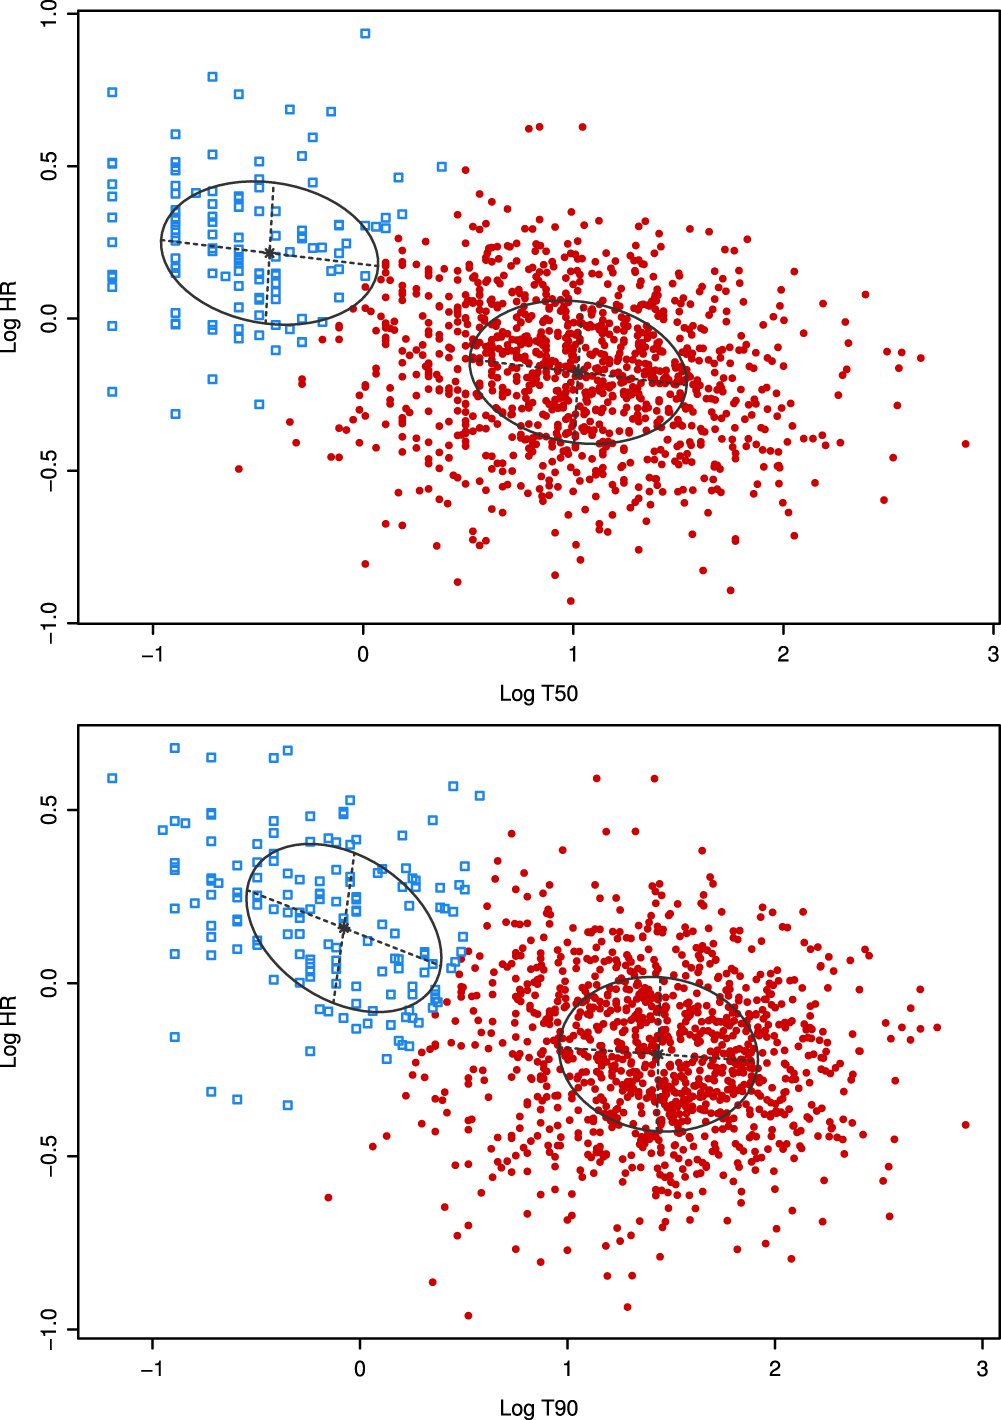
\includegraphics[trim={0 0 0 6cm}, clip, width=0.9\textwidth]{figures/gw/grb-classification.jpg}
	\caption{Hardness ratios (HR) vs. $T_{90}$s of Fermi GRBs, showing the distinction between short and long bursts. Reproduced from~\protect\citet{fermi_2016}}
	\label{fig:grb-classification}
\end{figure}

A multitude of models have been proposed throughout the decades to explain the origins of \acp{GRB}.
It is believed that the ultra-relativistic jets required to produce \acp{GRB} come from either black holes~\citep{Woosley_1993} or magnetars~\citep{Dai_1998}.
{\color{red}Go through a few more refs and review papers on GRB progenitors.}


\subsection{Short gamma-ray bursts}

\ac{GW} parameter estimation suffers from a degeneracy between distance and orbital plane inclination; increasing the distance of the merger and orienting its orbital plane would both result in a lower \ac{GW} amplitude.
This degeneracy can be broken if either one could be measured externally.
If the joint detection localization were good enough to determine a host galaxy, this would greatly help resolve the distance, however this will more likely require observation of an optical or UV counterpart due to the poor localization provided by current \ac{GRB} and \ac{GW} detectors.
In the case of GW170817, the host galaxy whose redshift was known was used to determine the distance, which then allowed for a more precise measurement of the inclination angle.
A separate analysis using the distance measured from the \ac{GW} detection combined with the known redshift made the first joint \ac{GW}-EM measurement of the Hubble constant, albeit with very large uncertainty due to the small sample size~\citep{gw170817_hubble}.

{\color{red}Discuss background and disagreement among Hubble constant measurements.}

One of the many unanswered questions surrounding \acp{GRB} pertains to their jet profile, the luminosity as a function of viewing angle (the angle between the observer and the symmetric axis of the jet; the profile is assumed to be axially symmetric and independent of distance).
When information about the jet profile is required, e.g. for making rate estimates for \ac{GRB} detections, the profile is typically modeled as a top-hat (uniform within some opening angle and dropping sharply beyond it) for simplicity, but the true profile may be different.

Determining the viewing angle $\theta_{\mathrm{obs}}$ of a \ac{GRB} is essential for distinguishing between different jet profile models, but it relies on the ability to observe an afterglow emission.
These emissions, ranging from radio to X-rays, follow the prompt emission of $\gamma$-rays and are generated by the interaction between the relativistic outflow and the surrounding medium.
The observation of these afterglows was crucial in improving localization of the \ac{GRB} sources and provided valuable information about the energy scale of the jet, as well as measurements of $\theta_{\mathrm{obs}}$.
The latter came from observing the signature jet break in the afterglow light curve, resulting from the lateral spreading of jet material as it expands; the opening angle can be determined from the timing of the jet break.
However, few jet breaks have been observed for short \acp{GRB}, so existing observations do not place tight constraints on opening angle~\citep{Biscoveanu_2020}.

Joint GW-GRB observations can provide much more information on jet properties~\citep{Mogushi_2019, Farah_2020}.
GRB170817 was orders of magnitude less energetic than most short \acp{GRB}, so it likely would have been ignored in the absence of a \ac{GW} coincidence.
Its low luminosity immediately ruled out an on-axis top-hat jet.
An off-axis top-hat jet was considered unlikely as well because the narrow opening angle predicted for top-hat jets based on theory and past \ac{GRB} measurements only allowed for $\theta_{\mathrm{obs}} \lesssim 10\deg$.
More evidence against an off-axis top-hat model arose when the bright afterglow expected to emerge after $\sim$1 day was not observed.
These observations instead favored a wide-angled, structured jet model for GRB170817.
A structured jet model may refer to any luminosity function that decreases gradually with $\theta_{\mathrm{obs}}$ rather than abruptly, e.g. a Gaussian or power-law with uniform center.
One mechanism that would explain such a model is a cocoon emission, in which the relativistic jet interacts dissipatively with the surrounding merger ejecta, depositing its energy into a cocoon fireball that results in a structured jet~\citep{gw170817_grb}.

The connection between GWs and short GRBs may extend beyond binary neutron star systems like GW170817.
Some \ac{NSBH} mergers may be capable of producing GRBs in the right conditions.
A mass ratio between the black hole and the neutron star is not too unequal, due to a low black hole mass, and a high prograde black hole spin could result in the \textit{tidal disruption} of the neutron star, which would produce a short GRB in much the same way as in a \ac{BNS} merger.


\subsection{Long gamma-ray bursts}

Long GRBs are believed to come from \acp{CCSN}, which as discussed above have many models predicting GW emission.
The majority (about 70\%) of GRBs are long GRBs, so although the expected GW amplitudes are quite weak they present an abundance of electromagnetic sources that each hold the potential of a GW counterpart.
Since these events are also expected to emit neutrinos, as was the case during SN 1987A, they are the primary candidate for a potential triple-messenger detection in which GWs, EM waves, and neutrinos are all observed from the same source.

Some models predict GW emission would occur as a result of asymmetries in the core-collapse phase.
Such \acp{GW} would be short, lasting less than a second.
Extreme emission models predict a wide variety of signals, often longer in duration.
Matter surrounding the remnant of a \ac{CCSN} forms an accretion disk, in which turbulent behavior can arise.
For instance, instabilities in the accretion disk can lead to the formation of a clump of matter which can then migrate inwards, shedding angular momentum in the form of gravitational waves~\citep{Piro_2007}.
Disk fragments are eventually torn apart by tidal disruption as they get too close to the central black hole, placing a maximum limit on the duration of potential GW emissions.

In an even more extreme scenario, two clumps could form as compact objects that merge within the disk, producing a CBC-like chirp~\citep{vanPutten_2001, vanPutten_2004}.

Accretion disk instability models are particular interesting due to their potential connection to X-ray flares.
Many GRBs exhibit a diverse range of X-ray flaring behavior that could be attributed to disk fragments falling in at different times after the formation of the central black hole~\citep{Dallosso_2017}.

Some long GRBs may even originate from compact mergers: some short GRBs have been observed to exhibit extended emissions that can last much longer than the initial short GRB impulse~\citep{Norris_2006, vanPutten_2014}.
These, too, may be associated with X-ray flaring, as accretion disks formed around NSBH mergers could likewise produce infalling clumps~\citep{Mu_2018}.
These scenarios raise questions about the simplistic short/long classification of GRBs.






% \section{Multi-messenger astronomy}\label{sec:mma}
%
% In addition to being the first ever detection of a merger between two neutron stars, GW170817 made history as the first astronomical event observed by both gravitational waves and electromagnetic waves.
% This was a major step forward for the field of multi-messenger astronomy, in which the only joint detection until then was that of SN 1987A by electromagnetic and neutrino observatories~\citep{Hirata_1987, Bionta_1987, Alekseev_1988}.
% The combined localization of the LIGO-Virgo network and Fermi-GBM prompted a world-wide follow-up campaign from observatories across the electromagnetic spectrum.
% This led to identification of an optical counterpart near NGC 4993, which in turn allowed astronomers to make the first confirmed observation of a kilonova, the multi-band emission of electromagnetic waves resulting from the radioactive decay of r-process material formed and ejected in all directions by the merger.
%
% The connection between GWs and GRBs may extend beyond binary neutron star systems like GW170817.
% Some \ac{NSBH} mergers may be capable of producing GRBs in the right conditions.
% A mass ratio between the black hole and the neutron star is not too unequal, due to a low black hole mass, and a high prograde black hole spin could result in the \textit{tidal disruption} of the neutron star, which would produce a short GRB in much the same way as a in a \ac{BNS} merger.
%
% Whereas the GRBs associated with \acp{CBC} are believed to be those classified as \textit{short}, GRBs classified as \textit{long} are believed to come from \acp{CCSN}, which as discussed above have many models predicting GW emission.
% The majority (about 70\%) of GRBs are long GRBs, so although the expected GW amplitudes are quite weak they present an abundance of electromagnetic sources that each hold the potential of a GW counterpart.
% Since these events also are expected to emit neutrinos, and neutrinos have been observed from one nearby supernova, SN 1987A, marking the first joint detection between EM and neutrino observatories.
% Another nearby supernova would be the most likely candidate for a joint detection between all three branches of multi-messenger astronomy: GWs, EM waves, and neutrinos.
%
% There is clearly much to be gained by using the time and sky localizations of GRB observatories to conduct \textit{targeted} searches for GW signals that can be much more sensitive than the uninformed all-sky searches.
